%Este trabalho está licenciado sob a Licença Atribuição-CompartilhaIgual 4.0 Internacional Creative Commons. Para visualizar uma cópia desta licença, visite http://creativecommons.org/licenses/by-sa/4.0/deed.pt_BR ou mande uma carta para Creative Commons, PO Box 1866, Mountain View, CA 94042, USA.

\chapter{Sistema de coordenadas}\label{cap_scoord}
\thispagestyle{fancy}

A geometria analítica é uma área interdisciplinar da matemática que faz o estudo de objetos da geometria através de estruturas algébricas (equações e inequações algébricas). Para tanto, o primeiro passo é a construção (definição) de um sistema de coordenadas, no qual os objetos geométricos serão referenciados.

\section{Sistema de coordenadas no espaço}\label{cap_scoord_sec_scoord}

\begin{flushright}
  \href{https://archive.org/details/sistema-de-coordenadas-tridimensional}{$\blacktriangleright$ Vídeo disponível!}
\end{flushright}

Um sistema de coordenadas no espaço (euclidiano) é constituído de um ponto $O$ e uma base de vetores $B = (\vec{e}_1, \vec{e}_2, \vec{e}_3)$ no espaço. Dado um tal sistema, temos que cada ponto $P$ determina de forma única um vetor $\overrightarrow{OP} = (x,y,z)$ e vice-versa. Assim sendo, definimos que o ponto $P$ tem coordenadas $(x,y,z)$. Veja a figura abaixo.

\begin{figure}[H]
  \centering
  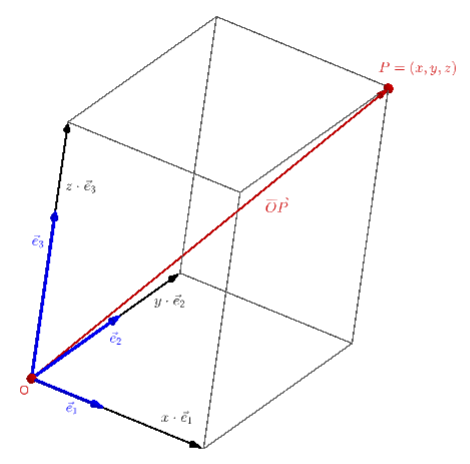
\includegraphics[width=0.8\textwidth]{cap_scoord/dados/fig_scoord/fig}
  \caption{Ilustração de um sistema de coordenadas no espaço.}
  \label{fig:scoord}
\end{figure}

O ponto $O$ é chamado de \emph{origem} (do sistema de coordenadas) e tem coordenadas $O=(0,0,0)$. Dado um ponto $P=(x,y,z)$, chama-se $x$ de sua \emph{abscissa}, $y$ de sua \emph{ordenada} e $z$ de sua \emph{cota}. As retas que passam por $O$ e têm, respectivamente, as mesmas direções de $\vec{e}_1$, $\vec{e}_2$ e $\vec{e}_3$ são chamadas de \emph{eixo das abscissas}, \emph{eixo das ordenadas} e \emph{eixo das cotas}. Os planos que contém $O$ e representantes de dois vetores da base $B$ são chamados de \emph{planos coordenados}.

\begin{figure}[H]
  \centering
  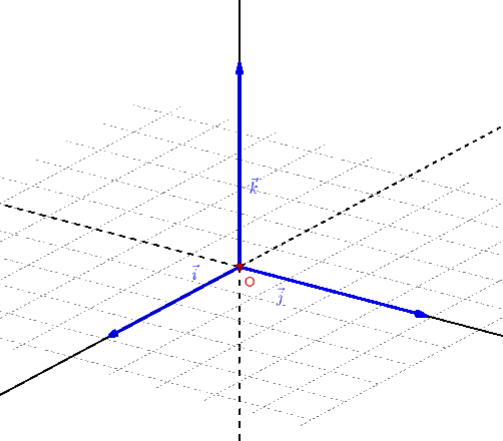
\includegraphics[width=0.7\textwidth]{./cap_scoord/dados/fig_sis_coord_orto/fig}
  \caption{Ilustração de um sistema de coordenadas ortonormal.}
  \label{fig:sis_coord_orto}
\end{figure}

Salvo explicitado ao contrário, trabalharemos com um \emph{sistema de coordenadas ortonormal}, i.e. sistema cuja base $B = (\vec{i},\vec{j},\vec{k})$ seja ortonormal. Mais ainda, estaremos assumindo que a base é positiva. Veja a Figura \ref{fig:sis_coord_orto}.

\begin{obs}\normalfont{(Relação entre pontos e vetores)(\href{https://archive.org/details/coordenadas-de-um-vetor}{$\blacktriangleright$ Vídeo disponível!})}
  Seja dado um vetor $\overrightarrow{AB}$. Sabendo as coordenadas dos pontos $A = (x_A,y_A,z_A)$ e $B = (x_B,y_B,z_B)$, temos que as coordenadas do vetor $\overrightarrow{AB}$ são:
  \begin{align}
    \overrightarrow{AB} &= \overrightarrow{AO} + \overrightarrow{OB}\\
                        &= -\overrightarrow{OA} + \overrightarrow{OB}\\
                        &= -(x_A,y_A,z_A)+(x_B,y_B,z_B)\\
                        &= (x_B-x_A,y_B-y_A,z_B-z_A).
  \end{align}
  Em uma linguagem menos formal, podemos dizer que as coordenadas de $\overrightarrow{AB}$ é a resultante das coordenadas do ponto final menos as coordenadas do ponto de partida. Veja a figura abaixo.

\begin{figure}[H]
  \centering
  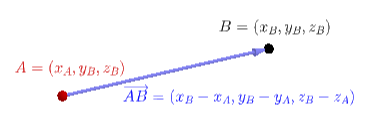
\includegraphics[width=0.6\textwidth]{./cap_scoord/dados/fig_scoord_vec_pt/fig}
  \caption{Relação entre as coordenadas dos pontos de partida e de chegada de um vetor.}
  \label{fig:scoord_vec_pt}
\end{figure}  
\end{obs}

\begin{ex}
  Dados os pontos $A = (-1,1,2)$ e $B = (3,-1,0)$, temos que o vetor $\overrightarrow{AB}$ tem coordenadas:
  \begin{equation}
    \overrightarrow{AB} = (3-(-1),-1-1,0-2) = (4,-2,-2).
  \end{equation}
\end{ex}

\begin{obs}\normalfont{(Ponto médio de um segmento)(\href{https://archive.org/details/coordenadas-do-ponto-medio}{$\blacktriangleright$ Vídeo disponível!})}
  Dados os pontos $A = (x_A,y_A,z_A)$ e $B = (x_B,y_B,z_B)$, podemos calcular as coordenadas do ponto médio $M = (x_M,y_M,z_M)$ do segmento $AB$. Veja a figura abaixo.

\begin{figure}[H]
  \centering
  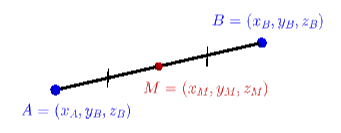
\includegraphics[width=0.6\textwidth]{./cap_scoord/dados/fig_scoord_pm/fig}
  \caption{Coordenadas do ponto médio de um segmento.}
  \label{fig:scoord_pm}
\end{figure}  

  Do fato de que $\overrightarrow{AM} = \overrightarrow{MB}$, temos
  \begin{equation}
    (x_M-x_A,y_M-y_A,z_M-z_A)=(x_B-x_M,y_B-y_M,z_B-z_M),
  \end{equation}
  Logo, segue que
  \begin{align}
    x_M-x_A &= x_B-x_M\\
    y_M-y_A &= y_B-y_M\\
    z_M-z_A &= z_B-z_M
  \end{align}
  ou, equivalentemente,
  \begin{align}
    2x_M &= x_A+x_B\\
    2y_M &= y_A+y_B\\
    2z_M &= z_A+z_B
  \end{align}
  Portanto, concluímos que
  \begin{align}
    x_M &= \frac{x_A+x_B}{2}\\
    y_M &= \frac{y_A+y_B}{2}\\
    z_M &= \frac{z_A+z_B}{2}
  \end{align}  
  Logo, temos
  \begin{equation}
  M = \left(\frac{x_A+x_B}{2},\frac{y_A+y_B}{2},\frac{z_A+z_B}{2}\right)
\end{equation}
\end{obs}

\begin{ex}
  Dados os pontos $A = (-1,1,2)$ e $B = (3,-1,0)$, temos que o ponto médio do segmento $AB$ tem coordenadas:
  \begin{align}
    M &= \left(\frac{-1+3}{2},\frac{1+(-1)}{2},\frac{2+0}{2}\right)\\
    &= (1,0,1).
  \end{align}
\end{ex}

\subsection*{Exercícios resolvidos}

\begin{exeresol}
  Sejam $A = (-1,2,1)$, $B = (1,-2,0)$ e $C = (x,2,2)$ vértices consecutivos de um triângulo isósceles, cujos lados $AC$ e $BC$ são congruentes. Determine o valor de $x$.
\end{exeresol}
\begin{resol}
  Sendo os lados $AC$ e $BC$ congruentes, temos $|\overrightarrow{AC}| = |\overrightarrow{BC}|$. As coordenadas de $\overrightarrow{AC}$ são
  \begin{equation}
    \overrightarrow{AC} = (x-(-1),2-2,2-1) = (x+1,0,1)
  \end{equation}
  e as coordenadas de $\overrightarrow{BC}$ são
  \begin{equation}
    \overrightarrow{BC} = (x-1,2-(-2),2-0) = (x-1,4,2).
  \end{equation}
  Então, temos
  \begin{align}
    |\overrightarrow{AC}| = |\overrightarrow{BC}| &\Rightarrow \sqrt{(x+1)^2+0^2+1^2} = \sqrt{(x-1)^2+4^2+2^2}\\
                                                  &\Rightarrow (x+1)^2+0^2+1^2 = (x-1)^2+4^2+2^2\\
                                                  &\Rightarrow x^2+2x+1+1 = x^2-2x+1+16+4\\
                                                  &\Rightarrow 4x = 19\\
                                                  &\Rightarrow x = \frac{19}{4}.
  \end{align}
\end{resol}

\begin{exeresol}
  Sejam $A = (-1,2,1)$, $B = (1,-2,0)$  e $M$ o ponto médio do intervalo $AB$. Determine as coordenadas do ponto $P$ de forma que $2AP = AM$.
\end{exeresol}
\begin{resol}
  As coordenadas do ponto médio são
  \begin{equation}
    M = \left(\frac{-1+1}{2},\frac{2+(-2)}{2},\frac{1+0}{2}\right) = \left(0,0,\frac{1}{2}\right).
  \end{equation}
  Agora, denotando $P = (x_P,y_P,z_P)$, temos
  \begin{align}
    2AP = AM &\Rightarrow 2(x_P-(-1),y_P-2,z_P-1) = \left(0-(-1),0-2,\frac{1}{2}-1\right)\\
             &\Rightarrow (2x_p+2,2y_P-4,2z_P-2) = \left(1,-2,-\frac{1}{2}\right).
  \end{align}
  Portanto
  \begin{align}
    & 2x_P+2 = 1 \Rightarrow x_P = -\frac{1}{2}\\
    & 2y_P-4 = -2 \Rightarrow y_P = 1\\
    & 2z_P-2 = -\frac{1}{2} \Rightarrow z_P = \frac{3}{4}.
  \end{align}
  Logo, $P = (-1/2,1,3/4)$.
\end{resol}

\subsection*{Exercícios}

\begin{exer}
  Sejam dados os pontos $A=(1,-1,2)$ e $B=(0,1,-2)$. Determine as coordenadas do vetor $\vec{v}=\overrightarrow{BA}$.
\end{exer}
\begin{resp}
  $\vec{v}=(1,-2,4)$
\end{resp}

\begin{exer}
  Sejam dados os pontos $E=(-1,2,0)$ e $F=(2,-1,1)$. Calcule o ponto médio do segmento $EF$.
\end{exer}
\begin{resp}
  $\displaystyle M=\left(\frac{1}{2},\frac{1}{2},\frac{1}{2}\right)$
\end{resp}

\begin{exer}
  Sejam dados os pontos $A=(-1,1,-1)$ e $M=(0,1,3)$. Determine o ponto $B$ tal que $M$ seja o ponto médio do segmento $AB$.
\end{exer}
\begin{resp}
  $B=(1,1,7)$
\end{resp}

\begin{exer}
  Sejam dados os pontos $A=(1,-1,1)$, $B=(2,1,0)$ e $C=(x,2,1)$. Determine $x$ tal que $ABC$ forme um triângulo retângulo com hipotenusa $BC$.
\end{exer}
\begin{resp}
  $x=-5$
\end{resp}

\begin{exer}
  Determine a distância entre os pontos $C=(2,-1,0)$ e $D=(1,1,1)$.
\end{exer}
\begin{resp}
  $|CD|=\sqrt{6}$
\end{resp}